\section{From Equilibria to Attacks}
\label{sec:attacks}

The equilibrium analysis treats every player as ordinarily
self-interested. This section turns the malice weight back on and
works out the attack picture that \cref{cor:coalition-attack}
predicts---and its two qualifications, both of which matter for threat
modelling: the attack presumes a victim who does not respond, and an
attacker who plays a repeated game does not attack at the minimum
budget. Every attack quantity in this section is a level-2 advantage
in the sense of \eqref{eq:hierarchy}: what the coalition moves is the
mechanism-specific bound on any adversary's advantage against the
resulting mechanism---the attack manipulates the mechanism, not the
attack tooling---so raising it raises the ceiling on every downstream
attacker at once.

\subsection{Coordination amplifies the externality against a passive
target}
\label{sec:C4}

We instantiate \cref{cor:coalition-attack} with five symmetric
players, the target pinned at $\eps_t = 32$ (the oblivious-victim
threat model of \citet{kaiser2026your}), non-colluders passive at
$\eps = 32$, and a coalition of $k$ players committing to the single
budget that maximises the target's realised advantage.

The target's advantage climbs monotonically and steeply in coalition
size (\cref{fig:C4}): $\Apld{t} = 0.442$ with no coalition, $0.483$,
$0.531$, $0.607$ at $k = 1, 2, 3$, and $0.728$ at $k = 4$---a $65\%$
inflation over baseline, mirroring the empirical attack success
reported by \citet{kaiser2026your}. The coalition's optimal budget
tracks the participation-preserving minimum of
\cref{cor:coalition-attack}: $\eps_C \approx 6.8$ for $k \le 3$,
relaxing to $\eps_C \approx 3.2$ at $k = 4$ as the collective batch
constraint slackens. The strategic content is the recovery, not the
curve: this is what \emph{any} coordinated subset of data holders
does if its joint utility weights the target's harm, no adversary
model required.

\begin{figure}[!t]
\centering
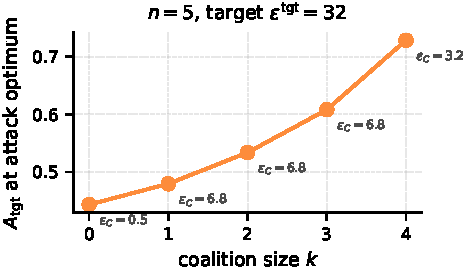
\includegraphics[width=\linewidth]{figures/fig_C4_coalition.pdf}
\caption{\textbf{Coalition attack against a passive target} ($n=5$,
target pinned at $\eps_t = 32$). Target's realised \ac{MIA} advantage
versus coalition size $k$, with the coalition playing its
target-maximising joint budget (annotated). The curve realises
\cref{cor:coalition-attack}: monotone in $k$, reaching $\Apld{t} = 0.728$
($+65\%$ over the $k{=}0$ baseline) at $k = 4$.}
\label{fig:C4}
\end{figure}

\subsection{The attack collapses against an aware target}
\label{sec:H4}

Pinning the target is the right model for an oblivious victim, but it
is not the game: an aware target sees the coalition's budgets and can
react. We rerun the same scenario with the target as a Stackelberg
follower, best-responding on a $14$-point log grid to whatever the
coalition commits, all else unchanged.

The attack collapses (\cref{fig:H4}). Across $k \in \{1,2,3,4\}$ the
aware target's realised advantage is $\Apld{t}^\star \in \{0.014, 0.010,
0.018, 0.041\}$---$18$--$53\times$ below the passive-target curve and
an order of magnitude below even the no-coalition baseline. For $k
\le 3$ the leader budget stays interior or at the loose ceiling
($\eps_C^\star \in \{44.1, 6.8, 64\}$) while the target retreats to
$\eps_t^\star \in [6.8, 14.4]$, where the mechanism-side externality
on their advantage is small. At $k = 4$ the leader argmax moves to
the grid floor---a \emph{poisoning corner} at $\eps_C = 0.5$ that
drags the target down to $\eps_t^\star = 0.73$---but even this
corner yields only $\Apld{t}^\star = 0.041$ while collapsing the
model utility the coalition itself trains for; the interior
optimum, continuous with $k \le 3$, does even less for the attacker
(\cref{fig:H4}, hollow marker). The reading for
threat modelling is sharp: the coalition attack is an attack on
\emph{unawareness}. Its empirical force in prior work comes from
targets that hold their budget fixed---rational for a
nominal-information player, per \cref{rem:awareness}---and a single
round of informed best response recovers almost the entire loss.
Disclosure of the mechanism's coupling to contributors is therefore
not just transparency hygiene; it is quantitatively the cheapest
defence available.

\begin{figure}[!t]
\centering
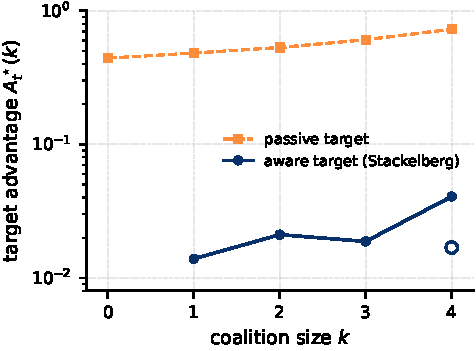
\includegraphics[width=\linewidth]{figures/fig_h4_aware_target.pdf}
\caption{\textbf{The coalition attack against an aware target}
(log-$y$). Orange squares: passive target pinned at $\eps_t = 32$
(as in \cref{fig:C4}), climbing to $\Apld{t} = 0.729$ at $k = 4$. Blue
circles: target best-responding to the coalition's commitment;
$\Apld{t}^\star \le 0.041$ throughout, $18$--$53\times$ below the
passive curve. At $k = 4$ the filled marker is the leader argmax (a
grid-floor poisoning corner that also ruins the coalition's own
utility); the hollow marker is the interior optimum that a
coalition with any self-interest plays.}
\label{fig:H4}
\end{figure}

\subsection{A repeated attacker learns the target---and does not play
the minimum budget}
\label{sec:brpeg}

Real deployments are repeated: budgets are re-declared, models
re-trained, and an attacker faces a target whose privacy preference it
does not know. We formalise the natural repeated extension---the
\emph{Bayesian Repeated PEG} (BR-PEG)---and extract its one
qualitative surprise. Two players: an attacker $M$ and an honest
target $H$ whose type $\theta_H = (\lambda_H, n_H)$ is drawn from a finite
set $\Theta$ known to $M$. Each round, $M$ commits to a budget
$\eps_M^t$; $H$ observes it and myopically best-responds; the
mechanism returns the round's outcomes, and $M$ Bayes-updates its
posterior over $\theta_H$ from $H$'s visible response. $M$'s score is
$\sum_t A_H^t$. The game is the Stackelberg-learning template of
\citet{letchford2009learning, blum2014learning, balcan2015commitment}
with the tabular follower payoff replaced by the \ac{DP} accountant, and
the myopic-informed case of repeated games with one-sided incomplete
information~\cite{aumann1995repeated}; \cref{app:bayesian} gives the
full formalism.

\begin{proposition}[The Bayesian-greedy attack is not min-budget]
\label[proposition]{prop:bayesian-not-min}
In the BR-PEG with $H$ myopic and $M$ posterior-greedy on a finite
action grid, suppose (I) the observation likelihood identifies
$\theta_H^\star$ on the equilibrium path~\cite{kalai1993rational} and
(A) the elicited-advantage map $G(\eps_M)$---the target's realised
advantage $A_H$ at the profile in which $M$ plays $\eps_M$ and $H$
plays $\eps_H^{\mathrm{BR}}(\eps_M; \theta_H^\star)$---has a unique
maximiser $\eps_M^\star > \eps^{\min}$. Then the
posterior-greedy action equals $\eps_M^\star$ for all sufficiently
large $t$, almost surely: the learned attack is bounded away from the
minimum budget.
\end{proposition}

The proof (\cref{app:bayesian}) is a uniform-convergence argument:
the posterior collapses on the true type, the posterior-averaged
score converges uniformly on the finite grid, and the argmax locks
onto the true-type optimum. The content is assumption (A) being
\emph{true} for the \ac{iDP} mechanism, which we verify numerically: the
advantage-maximising budget against a best-responding target is
interior because slamming $\eps_M$ to the floor drives $\sigma$ up
and pushes the target into retreat, whereas a moderate $\eps_M$
keeps the target comfortable at a budget whose realised advantage the
externality then inflates. In the canonical instance the oracle
attack sits at $\eps_M^\star \approx 3.2$ and elicits $A_H \approx
0.454$ per round---roughly twice the naive minimum-budget attack and
fifty times the benign baseline (\cref{app:bayesian}).

Learning speed is the remaining question: how much does not knowing
$\theta_H$ cost? \Cref{fig:regret} reports cumulative regret against
the full-information oracle on a harder instance designed to make
identification non-trivial (five overlapping types whose best
responses coincide at some arms, observation noise on $H$'s reported
utility, $40$ seeds, $T = 60$). The posterior-greedy attacker with a
correctly specified prior pays a bounded, front-loaded cost
($R(60) = 1.31 \pm 0.26$, flattening after roughly ten
identification rounds), while both non-learning baselines pay
linearly growing regret (uniform-belief $8.3$, misspecified prior
locked on a wrong type $8.4$ at $T = 60$) and a prior-free
adversarial bandit (EXP3~\cite{auer2002nonstochastic}) pays $13.2$.
For defenders the message is unpleasant but crisp: type uncertainty
is not a durable shield---a Bayesian attacker converts it into a
constant, not a rate.

\begin{figure}[!t]
\centering
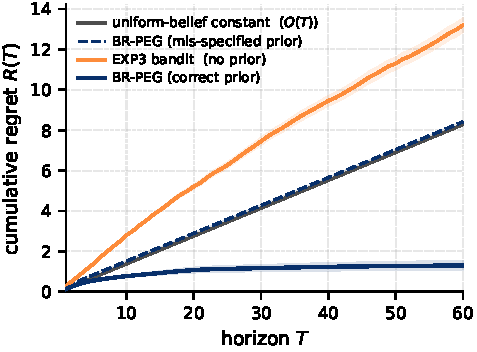
\includegraphics[width=0.9\linewidth]{figures/fig_h8_brpeg_regret.pdf}
\caption{\textbf{Cumulative regret of repeated attackers} against the
full-information Stackelberg oracle ($5$ overlapping target types,
noise of standard deviation $0.15$ on the target's observed
utility, $7$-arm budget grid, mean $\pm 1$\,SE over $40$ seeds). The posterior-greedy BR-PEG
attacker with a correct prior plateaus ($R(60) = 1.31$); a
misspecified prior and a static uniform belief pay linear regret
($8.4$ and $8.3$); the prior-free EXP3 bandit pays $13.2$. Learning
the target's type costs the attacker a constant, not a rate.}
\label{fig:regret}
\end{figure}
